\normaltrue \difficilefalse \tdifficilefalse
\correctionfalse

%\UPSTIidClasse{11} % 11 sup, 12 spé
%\newcommand{\UPSTIidClasse}{12}

\exer{Disque $\star\star$ \label{B2:10:45}}
\setcounter{question}{0}\UPSTIcompetence[2]{B2-10}
\index{Compétence B2-10}
\index{Disque}
\ifcorrection
\else
\marginnote{\textbf{Pas de corrigé pour cet exercice.}}
\fi




\ifprof
\else
Soit un secteur de disque de rayon $R$, d'épaisseur négligeable et de masse surfacique $\mu$. Il est percé d'un trou de rayon $r$ tel que $\vect{OA}=\dfrac{3}{4}R\vect{x}$.
\begin{figure}[H]
\centering
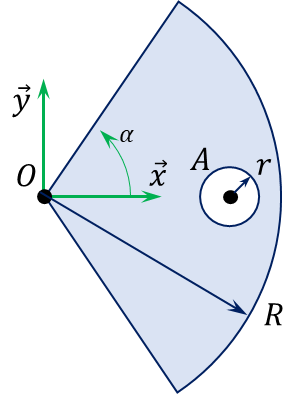
\includegraphics[width=.5\linewidth]{45_01}
\end{figure}
\fi


\question{Déterminer la position du centre d'inertie $G$ du solide.}
\ifprof
\else
\fi

\question{Déterminer la matrice d'inertie du solide en $O$.}
\ifprof ~\\
\else
\fi


\ifprof
\else
\begin{flushright}
\footnotesize{Corrigé voir \ref{B2:10:45}.}
\end{flushright}%
\fi